
% \vspace{-2em}
\section{Methodology} 
% \vspace{-1em}

In this section, we detail the proposed \textbf{C}onditional \textbf{Li}kelihood \textbf{D}iscrepancy (\textbf{CLiD}) method. We first introduce the threat model of query-based membership inference in \cref{sec:threat_m}. We then identify the conditional overfitting phenomenon with experimental validation in \cref{sec:key_i}. We further drive the membership inference indicator based on CLiD in \cref{sec:clid} and design two practical membership inference methods in \cref{sec:clid_mi}.
We finally provide the implementation details in \cref{sec:prac}.

\vspace{-2pt}
\subsection{Threat Model}\label{sec:threat_m}
\vspace{-2pt}

We use the standard security game of membership inference on image-text data following previous work \cite{sablayrolles2019white, carlini2022membership, carlini2023extracting, matsumoto2023membership}.
We define a challenger $\mathcal{C}$  and an adversary $\mathcal{A}$ who performs membership inference. $\mathcal{C}$ samples a member set $D_{\text{mem}} \leftarrow \mathbb{D}$ and trains or fine-tunes a text-to-image diffusion model $f_{\theta}$ (i.e., target model) with $D_{\text{mem}}$. The rest of $\mathbb{D}$ is denoted by hold-out set $D_{\text{out}}$ =  $\mathbb{D} \setminus D_{\text{mem}}$. 
For a given data point ${(\mathbf{x}, \mathbf{c}}) \in \mathbb{D} $, $\mathcal{A}$ designs an algorithm $\mathcal{M}$ to yield a membership prediction:
\begin{equation}  %\label{eq:mi_vec}
\mathcal{M}(\mathbf{x},\mathbf{c},f_{\theta}) = \mathbbm{1} \left[
\mathcal{M'}(\mathbf{x},\mathbf{c},f_{\theta})
> \tau  \right],
\end{equation}
where $\mathcal{M'}$ denotes an indicator function that reflects membership information, and $\tau $ denotes a tunable decision threshold of query-based membership inference \cite{matsumoto2023membership,duan2023diffusion, kong2023efficient,fu2023probabilistic}.


We consider a grey-box setting
\footnote{Note that in most real-world scenarios, the requirements for  $\mathcal{A}$ in gray-box and white-box settings are nearly identical. We use this terminology here for consistency with previous works~\cite{duan2023diffusion, kong2023efficient}.} 
consistent with previous query-based methods \cite{matsumoto2023membership,duan2023diffusion, kong2023efficient, fu2023probabilistic}. This setting assumes that  $\mathcal{A}$ has access to the intermediate outputs of models without knowledge of specific model parameters.
For the given image-text data point $(\mathbf{x}, \mathbf{c})$, we assume that $\mathbf{x}$ and $\mathbf{c}$ always correspond within the dataset $\mathbb{D}$. This assumption is evident in scenarios where dataset copyright owners perform membership inference to audit usage. And we also consider a weaker assumption of conducting membership inference without the groundtruth text in Sec.~\ref{sec: weak_assumption}.

Conversely, challenger $\mathcal{C}$ can mitigate the effectiveness of membership inference during training by utilizing data augmentation or even adaptive defense methods, which we discuss in Sec.~\ref{sec:defense}. Our work primarily focuses on fine-tuning scenarios because the weights of pretrained models are readily available, making this scenario more prone to copyright risks \cite{wang2023diagnosis, pang2023black}. Numerous projects are implemented by fine-tuning open-source models on specific datasets~\cite{text-to-image-ft, FT-CLOOB-Conditioned, Heart-of-Apple-XL, yeh2023navigating}.
We also conduct experiments on pretrained text-to-image diffusion models (Tab.~\ref{tab:wrap_pretrain}) to demonstrate the effectiveness of our method even in pretraining scenarios.

\subsection{Conditional Overfitting Phenomenon}\label{sec:key_i}
The rationale behind previous studies primarily hinges on the overfitting of diffusion models to training data (usually image data $\mathbf{x}$)~\cite{matsumoto2023membership, duan2023diffusion, kong2023efficient,chen2023robust,chen2024your}. This overfitting tends to result in lower estimation errors for images in the member set (training data) compared to those in the hold-out set during the diffusion process. Various indicators~\cite{matsumoto2023membership, duan2023diffusion, kong2023efficient} are designed based on this to expose membership information.
Specifically, let $q_{\text{mem}}$ and $q_{\text{out}}$ represent the image distributions of the member set and the hold-out set, respectively.  \( p \) represents the diffusion models' estimated distribution, and $D$ denotes a distance metric (which will be specified later). This rationale can be formulated as:
%%%%%%%%%%%
\begin{equation}
    D(q_{\text{mem}}(\vect{x}), p(\vect{x}))  \leq 
    D(q_{\text{out}}(\vect{x}), p(\vect{x})).
\end{equation}
% \zsf{assumption?}
However, if considering the membership inference on text-to-image diffusion models with image-text data \((\vect{x}, \mathbf{c})\), we emphasize the following assumption:
\begin{assumption}[Conditional overfitting phenomenon] \label{theorem:assumption}
The overfitting of text-to-image diffusion models to the conditional distribution of \((\vect{x}, \mathbf{c})\) is more salient than to the marginal distribution of \(\vect{x}\):
\begin{equation}\label{eq:overfit_conditional}
     \underbrace{\mathbb{E}_{\mathbf{c}}[D(q_{\text{out}}(\vect{x}|\mathbf{c}), p(\vect{x}|\mathbf{c})) - D(q_{\text{mem}}(\vect{x}|\mathbf{c}), p(\vect{x}|\mathbf{c}))]}_{\text{overfitting to conditional distribution}}  
       \geq \underbrace{D(q_{\text{out}}(\vect{x}), p(\vect{x})) - D(q_{\text{mem}}(\vect{x}), p(\vect{x})) }_{\text{overfitting to marginal distribution}}.
\end{equation}
\end{assumption}
\begin{wrapfigure}[15]{r}{0.53\textwidth}
\vspace{-0.4cm}
\centering
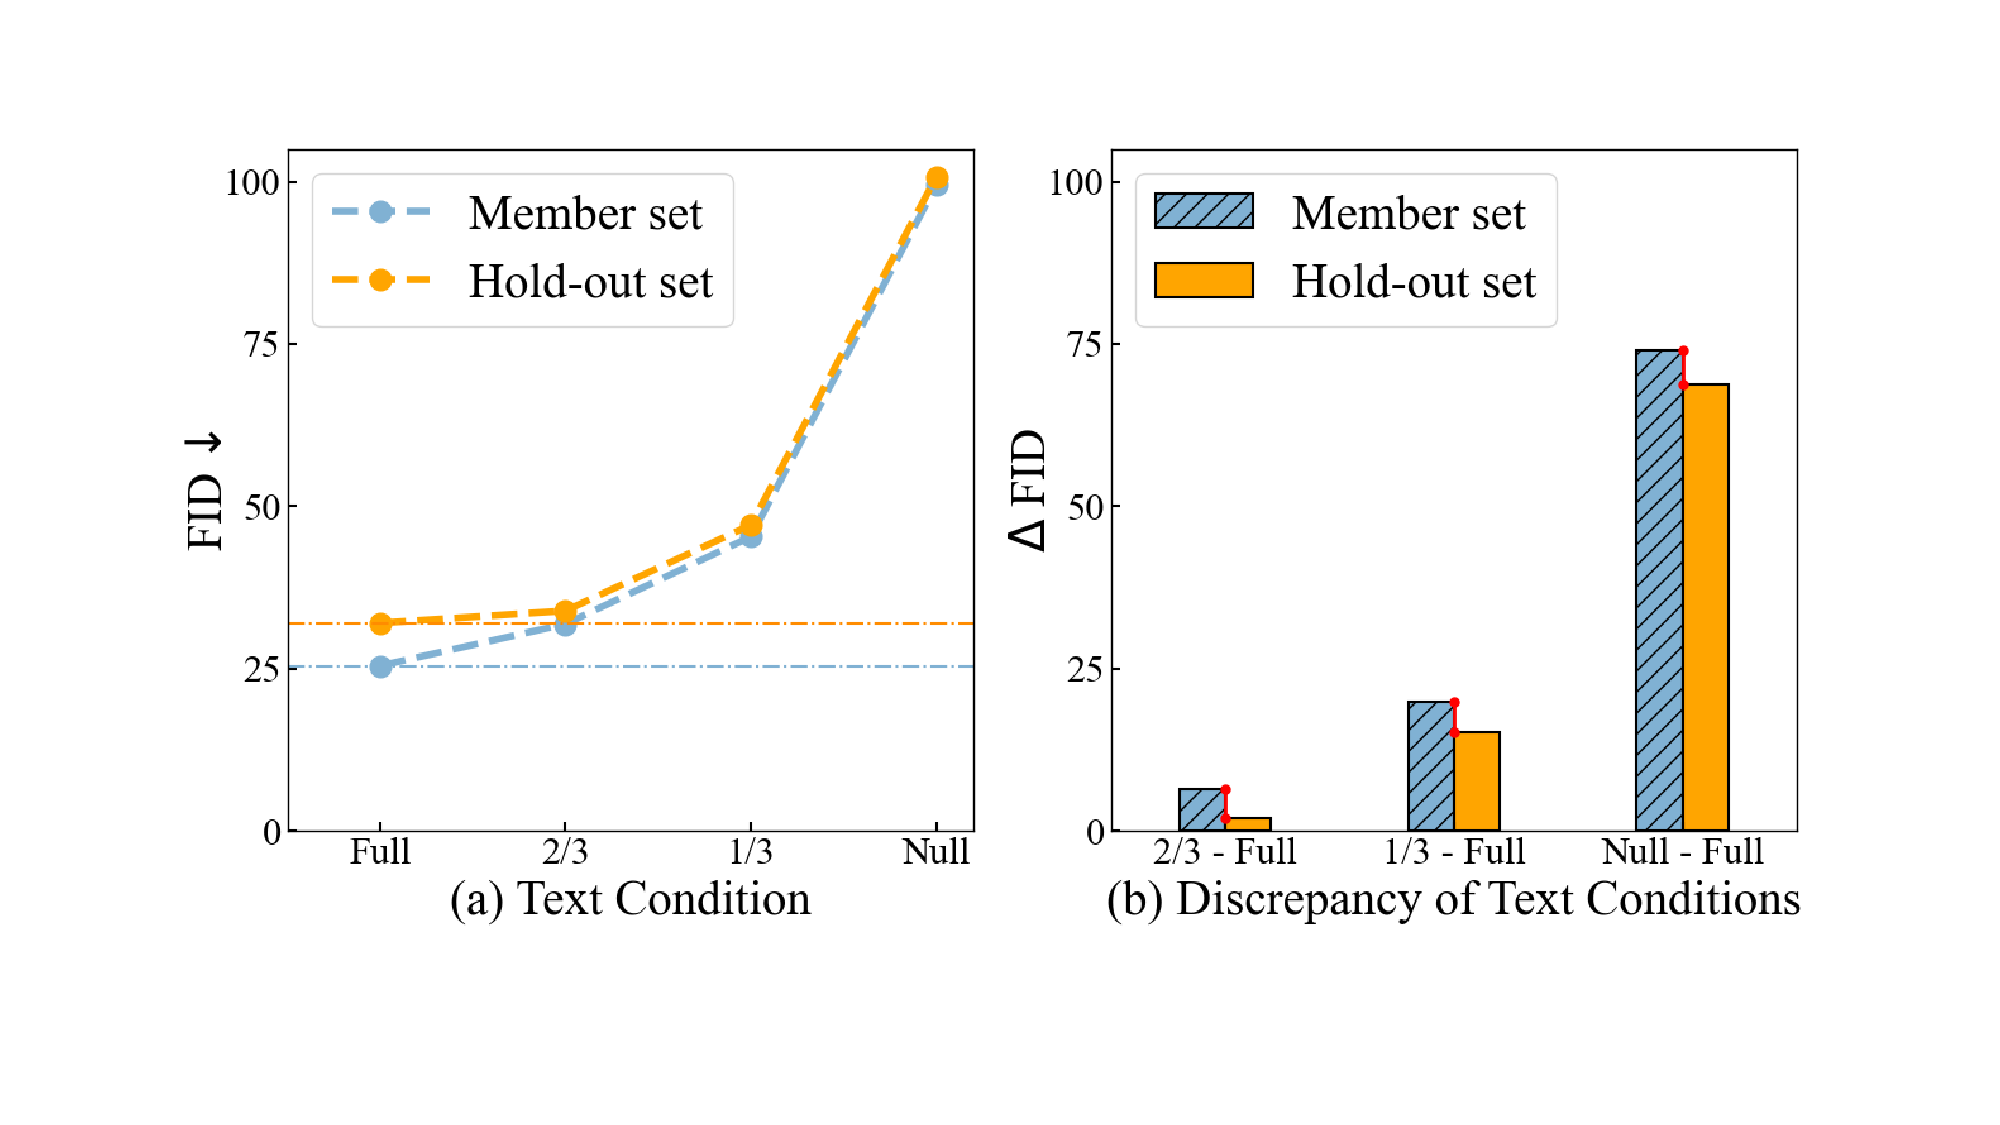
\includegraphics[scale=0.26]{imgs/intuition.pdf}
\caption{
FID values   and the FID differences
% and the difference 
of synthetic images ($2500/2500$ samples for member/hold-out set) under different conditions of member set and hold-out set.
}
\label{fig:intuition}
\end{wrapfigure}
Empirically, we validate this assumption by using Fréchet Inception Distance (FID)~\cite{heusel2017gans} as the metric $D$, i.e., \(D_{FID}\). 
We calculate $D_{FID}(q(\vect{x}|\mathbf{c}), p(\vect{x}|\mathbf{c}))$ using the  MS-COCO \cite{lin2014microsoft} dataset on a fine-tuned Stable Diffusion \cite{rombach2022high} model. Then by gradually truncating the original condition text to $\{2\big/3, 1\big/3, Null\}$ to obtain $\mathbf{c}^*$, we calculate $D_{FID}(q(\vect{x}|\mathbf{c}^*), p(\vect{x}|\mathbf{c}^*))$ as a stepwise approximation of  \(D_{FID}(q(\vect{x}), p(\vect{x}))\).
In Fig.~\ref{fig:intuition}, we report the FID scores of synthetic images under different conditions of member set and hold-out set. A smaller FID value indicates a closer match between model distributions and dataset distributions. 
From Fig.~\ref{fig:intuition} (a), it can be observed that for the full condition, the FID difference between the member set and the hold-out set is consistently higher than that for the truncated conditions, which validates our assumptions.  
We also demonstrate the validation utilizing other metrics in Appendix~\ref{appd:validation}.



We further compute the change in FID after truncating the condition and observe that the change in FID of the member set is consistently greater than that of the hold-out set (Fig.~\ref{fig:intuition} (b)), which inspires revealing membership 
by this overfitting discrepancy.
Recalling the aim of text-to-image diffusion model is to fit a latent space mapping from text to image, 
image data augmentation is commonly used to enhance the model generalization.
For instance, the official fine-tuning script of Hugging-Face~\cite{text-to-image-ft} employs Random-Crop and Random-Flip as the default augmentation \cite{text-to-image-ft-python}.
However, few trainers disturb the text condition as it is discrete and such disturbance would result in a decline of model utility (\cref{sec:defense}). 
Therefore, we believe that leveraging this phenomenon contributes to addressing the challenges of the strong generalization of text-to-image diffusion models with the resistance to data augmentation. 


\subsection{Condition Likelihood Discrepancy}\label{sec:clid}
In this section, we derive a membership inference indicator for a given individual sample based on Assumption~\ref{theorem:assumption}.
Calculating FID requires sampling lots of images from the $p$ distribution, 
which is impractical under membership inference scenarios.
Instead, we employ Kullback-Leibler (KL) divergence as the distance metric, which is widely used and computationally convenient 
(the usage of other metrics is discussed in Appendix~\ref{appd:other_metric}). Then we have the following theorem:

\begin{theorem}
\label{theorem:theorem}
(Proof in Appendix~\ref{appd: proof})
When using \(D=D_{KL}\) as distance metric, Assumption~\ref{theorem:assumption} is equivalent to:
\begin{equation}
\label{eq:theorem}
       \mathbb{E}_{q_{\text{mem}}(\vect{x}, \vect{c})}[\log p(\vect{x}|\vect{c}) - \log p(\vect{x})]
          \geq        
       \mathbb{E}_{q_{\text{out}}(\vect{x}, \vect{c})}[\log p(\vect{x}|\vect{c}) - \log p(\vect{x})]
       + \delta_{H},
\end{equation}
where
\begin{equation}
    \delta_H = H(q_{\text{out}}(\vect{x})) + \mathbb{E}_{\vect{c}}[H(q_{\text{mem}}(\vect{x}|\vect{c}))]
       - H(q_{\text{mem}}(\vect{x})) - \mathbb{E}_{\vect{c}}[H(q_{\text{out}}(\vect{x}|\vect{c}))].
\end{equation}
\end{theorem}


% ----------------------

Let us define: 
\begin{equation}\label{eq:indicator}
    \mathbb{I}(\mathbf{x},\mathbf{c}) = \log p(\vect{x} | \mathbf{c}) - \log p(\vect{x}).
\end{equation} 
If \(\delta_H\) is negligible, then according to \cref{eq:theorem}, it holds that \(\mathbb{E}_{q_{\text{mem}}}[\mathbb{I}(\mathbf{x})] \geq \tau \geq \mathbb{E}_{q_{\text{out}}}[\mathbb{I}(\mathbf{x})]\), where \(\tau\) is a constant intermediate between the left-hand side and right-hand side. 
Membership inference is then posed as follows: given an input instance \((\vect{x}, \mathbf{c})\), measuring \(\mathbb{I}(\mathbf{x}, \mathbf{c})\) to predict how probable it is that the input is a sample from \(q_{\text{mem}}\) rather than \(q_{\text{out}}\). 
Intuitively, if \(\mathbb{I}(\mathbf{x})\) exceeds a threshold \(\tau\), the instance is likely from \(q_{\text{mem}}\); otherwise, it belongs to \(q_{\text{out}}\). In the community of membership inference methods 
\cite{yeom2018privacy,chen2020gan,carlini2022membership, carlini2023extracting,matsumoto2023membership, duan2023diffusion, kong2023efficient, fu2023probabilistic}
, setting such a threshold \(\tau\) is a standard practice to differentiate between the two distributions. 
Therefore, we can utilize the indicator \(\mathbb{I}(\mathbf{x}, \mathbf{c})\) for membership inference.
Since Eq.~\eqref{eq:indicator}  actually involves measuring the likelihood discrepancy under different conditions of diffusion models, we call it \textbf{C}onditional \textbf{Li}kelihood \textbf{D}iscrepancy (\textbf{CLiD}).

In order to calculate the likelihoods in Eq.~\eqref{eq:indicator} for a given data point $(\mathbf{x},\mathbf{c})$, we utilize the ELBOs in Eq.~\eqref{eq:ddpm_elbo} and Eq.~\eqref{eq:cdm_elbo}  as an approximation of the log-likelihoods:
\begin{equation}\label{eq:CLiD_loss_ori}
     \mathbb{I}(\mathbf{x},\mathbf{c}) =
     \mathbb{E}_{ t, \mathbf{\epsilon}} \left[|| \mathbf{\epsilon}_{\theta}( \mathbf{x}_t    , t, \mathbf{c}_{\text{null}}) - \epsilon ||^2
     \right] 
     -  
     \mathbb{E}_{ t, \mathbf{\epsilon}} \left[
     || \mathbf{\epsilon}_{\theta}( \mathbf{x}_t    , t, \mathbf{c}) - \epsilon ||^2 \right],
\end{equation}
where $\mathbf{c}_{\text{null}}$ denotes an empty text condition input used to estimate the approximation of $\log p_\theta(\mathbf{x})$.


\subsection{Implementation of CLiD-MI}\label{sec:clid_mi}

In practice, calculating Eq.~\eqref{eq:CLiD_loss_ori} needs a Monte Carlo estimate for data point by 
sampling $N$ times using $(t_i, \epsilon_i)$
pairs, with $\epsilon_i \sim \mathcal{N}(\mathbf{0},\mathbf{I})$ and  $t_i \sim [1,1000] $. Performing two Monte Carlo estimations independently incurs high computational costs, resulting in $2 \times N$ query count, where  $N$ is typically a large number to ensure accurate estimation. To simplify computation, we instead perform Monte Carlo estimation on the difference of the ELBOs inspired by \cite{li2023your}:
\begin{equation}\label{eq:CLiD_loss}
    \mathbb{I}(\mathbf{x},\mathbf{c}) =
     \mathbb{E}_{ t, \mathbf{\epsilon}} \left[|| \mathbf{\epsilon}_{\theta}( \mathbf{x}_t    , t, \mathbf{c}_{\text{null}}) - \epsilon ||^2
     -  
     || \mathbf{\epsilon}_{\theta}( \mathbf{x}_t    , t, \mathbf{c}) - \epsilon ||^2 \right].
\end{equation}
In experiments, to further mitigate randomness, we also consider diverse reduced conditions along with  $\mathbf{c}_{\text{null}}$, forming the reduced condition set  
 $\mathbb{C} = \{\mathbf{c}^*_1, \mathbf{c}^*_2..., \mathbf{c}^*_{k}\}$, where we set 
 $\mathbf{c}^*_{k} = \mathbf{c}_{\text{null}}$. Then we compute multiple condition likelihood discrepancies:
\begin{equation}\label{eq:clid_loss_reduction}
    \mathcal{D}_{\mathbf{x},\mathbf{c},\mathbf{c}^*_i} = 
    \mathbb{E}_{ t, \mathbf{\epsilon}} \left[|| \mathbf{\epsilon}_{\theta}( \mathbf{x}_t    , t, \mathbf{c}^*_i) - \epsilon ||^2
     -  
     || \mathbf{\epsilon}_{\theta}( \mathbf{x}_t    , t, \mathbf{c}) - \epsilon ||^2 \right],
\end{equation}
where $\mathbf{c}_i^* \in \mathbb{C} $. In subsequent parts, we employ their mean or treat them as feature vectors to reveal membership information. We will introduce how to obtain $\mathbb{C}$ in \cref{sec:prac}.

\textbf{Combining $p_\theta(\vect{x}|\vect{c})$ for further enhancement.}
Recall that the practical significance of sample likelihood is the probability that a data point originates from the model distribution, which essentially can also be used to assess membership.
Due to the monotonicity of the log function, we can also use ELBO of Eq.~\eqref{eq:cdm_elbo} to estimate $p_\theta(\vect{x}|\vect{c})$:
\begin{equation}\label{eq:elbo_loss}
    \mathcal{L}_{\mathbf{x},\mathbf{c}} = - \mathbb{E}_{ t, \mathbf{\epsilon}} \left[|| \mathbf{\epsilon}_{\theta}( \mathbf{x}_t    , t, \mathbf{c}) - \epsilon ||^2 \right].
\end{equation}
Additionally, this estimation can reuse results from estimating Eq.~\eqref{eq:clid_loss_reduction}, thus obviating any additional query counts. Next, we consider two strategies to combine Eq.~\eqref{eq:clid_loss_reduction} and Eq.~\eqref{eq:elbo_loss} to construct the final membership inference method.

\textbf{Threshold-based attack--\clidth.}
First, we normalize the two indicators to the same feature scale. Due to the outliers in the data, we use Robust-Scaler: $\mathcal{S}(a_{i}) = (a_{i} - \tilde{a}) \big/ IQR $, where $a_{i}$ denotes the $i$-th value,  $\tilde{a}$ denotes the mean and IQR (interquartile range) is defined as the difference between the third quartile (Q3) and the first quartile (Q1) of the feature. Then we have:
\begin{equation}\label{eq:mi_th}
     \mathcal{M}_{\text{CLiD}_{th}}(\mathbf{x},\mathbf{c}) = \mathbbm{1} \left[
     \alpha \cdot \mathcal{S}(\frac{1}{k} \sum_{i}^{k}  \mathcal{D}_{\mathbf{x},\mathbf{c},\mathbf{c}^*_i})
     +
 (1-\alpha) \cdot \mathcal{S}(\mathcal{L}_{\mathbf{x},\mathbf{c}}) 
 > \tau  \right],
\end{equation}
where $k$ denotes the total number of reduced $\mathbf{c}^*$ (i.e., $k =  \left| \mathbb{C} \right|$),  and $\alpha$ is a weight parameter. 


\textbf{Vector-based attack--\clidvec.}
We combine the estimated values of Eq.~\eqref{eq:clid_loss_reduction} and Eq.~\eqref{eq:elbo_loss} to obtain the feature vectors corresponding to each data point:
\begin{equation}\label{eq:vec}
    \mathbf{V} = 
\begin{pmatrix}
\mathcal{D}_{\mathbf{x},\mathbf{c},\mathbf{c}^*_1},
\mathcal{D}_{\mathbf{x},\mathbf{c},\mathbf{c}^*_2} 
\hdots
\mathcal{D}_{\mathbf{x},\mathbf{c},\mathbf{c}^*_k},
\mathcal{L}_{\mathbf{x},\mathbf{c}}
\end{pmatrix}.
\end{equation}
We use a simple classifier to distinguish feature vectors in order to determine the membership of the samples: 
\begin{equation}\label{eq:mi_vec}
\mathcal{M}_{\text{CLiD}_{vec}}(\mathbf{x},\mathbf{c}) = \mathbbm{1} \left[
\mathcal{F}_{\mathcal{M}} % _{cls}
(
\mathbf{V}
)
> \tau  \right],
\end{equation}
where $\mathcal{F}_{\mathcal{M}}$ denotes the predict confidence of the classifier. 



\subsection{Practical Considerations}\label{sec:prac}

\textbf{Reducing conditions to obtain $\mathbf{c}^*$.} 
We consider three methods for diverse reduction:
(1) Simply taking the first, middle, and last thirds of the sentences as text inputs. (2) Randomly adding Gaussian noises with various scales to the text embeddings. (3) Calculating the importance of words in the text  \cite{tang2023daam, wang2024promptcharm} and replacing them with “pad” tokens by varying proportions in descending order. For all three methods, we additionally use the null text input as $\mathbf{c}^*_k$. These methods are all effective and we use (3) with $k=4$ in subsequent experiments (details in Appendix~\ref{appd:detail}).

\textbf{Monte Carlo sampling.}  \label{sec:mtcl_sample}
 Let $M$ and $N$ denote the Monte Carlo sampling numbers of estimating $\mathcal{L}(\mathbf{x},\mathbf{c})$ and $\mathcal{D}_{\mathbf{x},\mathbf{c},\mathbf{c}^*_i}$, respectively.
 We set $M=N$ to achieve result reuse between Eq.~\eqref{eq:clid_loss_reduction} and Eq.~\eqref{eq:elbo_loss}, reducing the number of Monte Carlo sampling.
 Hence the overall query count of one data point is $M + K \cdot N$. Significant effects can be observed even when $M, N = 1$ (Fig.~\ref{fig:auc_samples}).

\textbf{Classifiers of \clidvec.} 
 Due to the simplicity of the feature vectors, we do not need a neural network as the classifier \cite{duan2023diffusion}. Simpler classifiers help to prevent overfitting.
In our experiments, we utilize XGBoost~\cite{chen2016xgboost} and utilize its predict confidence.
